\documentclass{article}
\usepackage[margin=0.5in]{geometry}
\usepackage{hyperref}
\usepackage{titling}
\pretitle{% add some rules
  \begin{flushleft}
    \huge\bfseries
}
\posttitle{%
  \end{flushleft}
}
\renewcommand\maketitlehooka{%
	\vspace{-10ex}
  \noindent\vrule height 2.5pt width \textwidth
}
\renewcommand\maketitlehookb{%
  \begin{flushleft}
   \Large\bfseries
    Representative Work, 2021
  \end{flushleft}%
    \noindent\vrule height 2.5pt width \textwidth
}
\title{Shivesh Pathak}
\date{\vspace{-10ex}}
\usepackage{graphicx}
\usepackage{wrapfig}
\begin{document}
\maketitle

\section{Non-orthogonal multi-Slater-Jastrow wave functions in diffusion Monte Carlo}
\begin{wrapfigure}{r}{0.5\textwidth}
	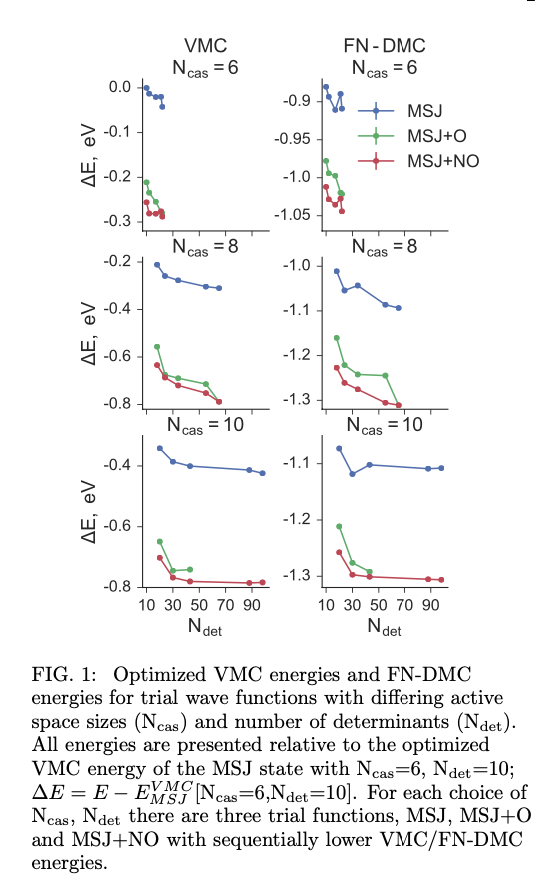
\includegraphics[width=0.48\textwidth]{nonortho.png}
\end{wrapfigure}
We investigated compact representations of ground state wave functions in QMC,  quantifying the benefit of using non-orthogonal orbitals in multi-Slater-Jastrow trial wavefunctions in QMC versus the traditional orthogonal orbitals (\textbf{Pathak}, Wagner,  J. Chem. Phys.  (2018)).
We computed the total energy of a $C_2$ molecule using both the orthogonal and non-orthogonal orbitals, and are presented in total energies are presented in Figure 1. 
We found that the traditional orthogonal orbitals (MSJ + O) yielded a significant decrease in total energy, of 0.14 eV on average.
The novel non-orthogonal optimization (MSJ + NO) improves the energy by a smaller amount of  0.03 eV on average, but still a significant contribution nonetheless.
This would actually be quite comparable to the energy scales we care about in condensed matter systems.
Recent publications on non-orthogonal configuration interaction have made use of our results (Burton \textit{et al.}, J. Chem. Theory and Comp. (2019, 2020)).

\section{A light weight regularization for wave function parameter gradients in quantum Monte Carlo}
In the process of constructing the wave functions for the first project, we found that certain gradients required in the optimization method had very large statistical variances,  leading to inhibitively long optimization times within QMC.
This infinite variance problem spawned a second methodology focused QMC project, where we identified and suggested a simple and efficient fix to the infinite variance problem in QMC when computing the total energy gradient required for wave function optimization (\textbf{Pathak}, Wagner, AIP Advances (2020)).
We showed that this infinite variance problem occurred when optimizing parameters that affected the nodal surface of the wave function, in particular orbital parameters - the parameters we were focused on in the first project.
We then suggested a simple fix by applying a regularization when computing the gradient in QMC,  proved mathematically that it leads to a finite variance estimate for the gradient, and implemented it and tested it on the CuO molecule.
In Figure 2, I show how the regularization clearly reduces the variance during wave function optimization relative to the bare estimator while performing comparably to state-of-the-art methods.
Our regularization method lead to a simple solution to a problem which was previously handled by complex methods using auxiliary wave functions, and served well for in the latter projects during my PhD which made heavy use of orbital optimization.
\begin{wrapfigure}{r}{0.5\textwidth}
	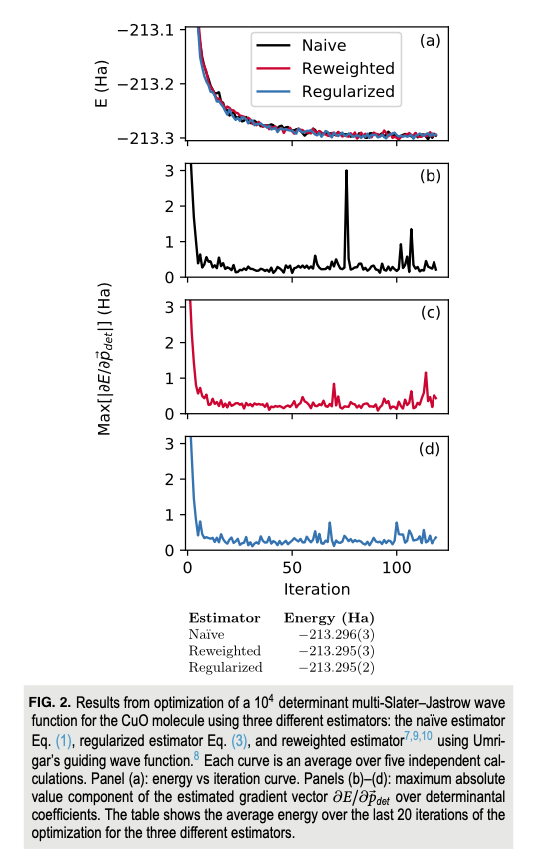
\includegraphics[width=0.48\textwidth]{pgrad.png}
\end{wrapfigure}

\section{Excited states in variational Monte Carlo using a penalty based method}
After these QMC methods based projects, my focus shifted towards model development using QMC calculations and the novel DMD method previously developed in Lucas Wagner's group.
DMD is a method which allows us to use total energies and density matrices computed from \textit{ab initio} simulations of low-energy states in condensed matter systems to fit effective atomic-scale models using statistical regression techniques.
Integral to this method is the efficient, accurate, and systematic computation of low-energy states: the accuracy of the low-energy states correlates with the accuracy of the fit model,  the more states that can be computed the lower the statistical uncertainty on the fit model, and having a systematic method allows for applications to a broad range of condensed matter systems.
Prior work with DMD has established that QMC methods serve as efficient and accurate techniques for computation, but no systematic method for computing low-energy states had existed.
The latter half of my PhD work has revolved around the development of such a systematic QMC method for computing low-energy states, and the application of the method in developing models for graphene based systems.

The systematic method that we developed is an extension of standard wave function energy optimization techniques in QMC by including an overlap penalty (\textbf{Pathak} \textit{et al.} J. Chem. Phys. (2020)).
The method allows us to target the lowest energy wave function with specified overlaps with other wave functions.
For example, the first excited state is computed by targeting the lowest energy wave function with zero overlap to the ground state, the second excited state as the lowest energy wave function with zero overlap to the ground and first excited states, and so on.
As such, we can conduct a ground state optimization using well established methods, and then use our new penalty based method to construct a tower of low-energy excited states in a systematic fashion that can be applied to any system.
We went on to apply this method to the benzene molecule, computing the entire $\pi$ active space spectrum, twelve excited states, and found agreement with experiment to 0.2 eV for all twelve states.
The computed values alongside other state-of-the art techniques is presented in Table 1.
The penalty-based method we developed clearly serves as an efficient, accurate, and systematic technique required for computing low-energy states for DMD.
\begin{wrapfigure}{r}{1.0\textwidth}
	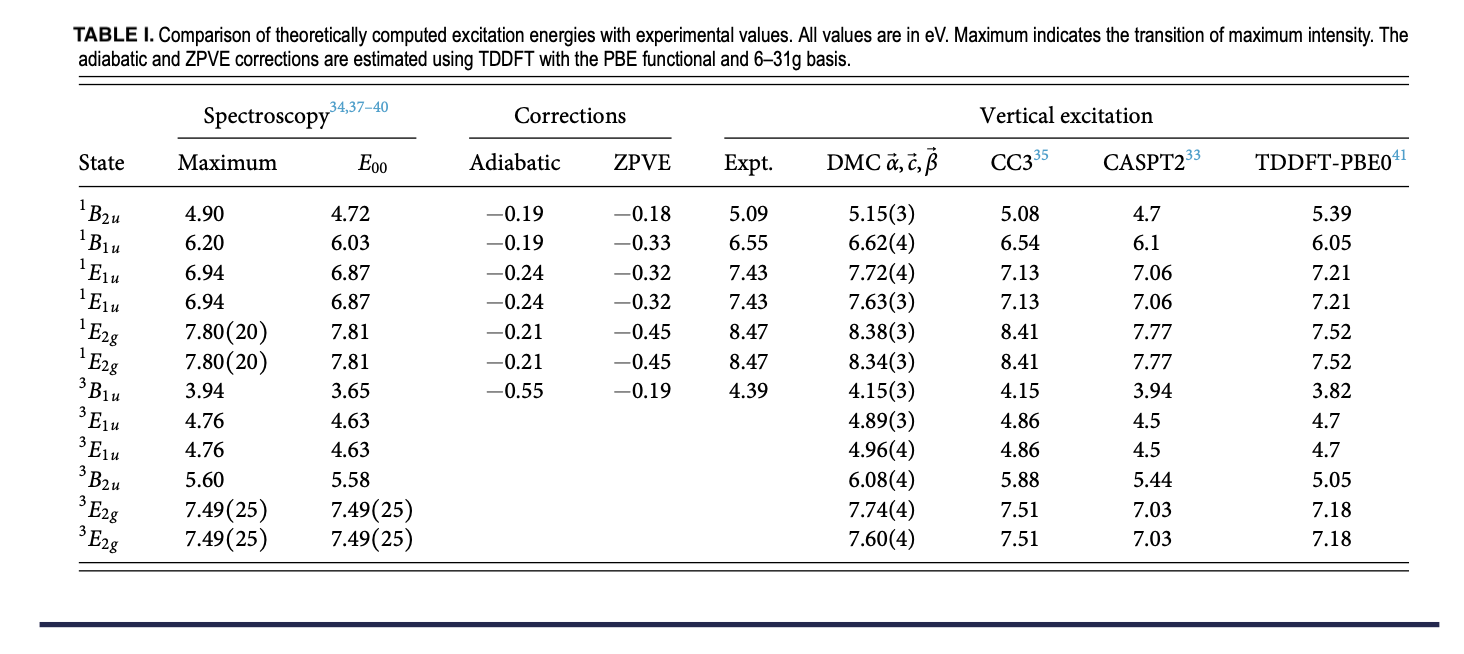
\includegraphics[width=0.98\textwidth]{benzene.png}
\end{wrapfigure}
\end{document}
